\chapter{Evaluation Supplementals}
\label{chapter:appendix_results}
%%%%%%%%%%%%%%%%%%%%%%%%%%%%%%%%%%%%%%%%%%%%%%%%%%%%%%%%%%%%%%%%%%%%%%%%%%%%%%%%%%%%%

\section*{\cottontail{} Entities \& Configuration}

\subsection*{Configuration Parameters}

\begin{lstlisting}[language=json, caption={Cottontail DB configuration used during evaluation (config.json).}, label=listing:cottontail_config, numbers=none]
{
    /* Path to data folder. */
    "root":"/mnt/raid0/evaluation/cottontail-data",
    "server": {
      /* Port used by gRPC query interface. */
      "port": 1865
    },
    "cost": {
      /* Allows for aggressive parallelisation. */
      "speedupPerWorker": 0.00,  

      /* Portion of IO costconsidered parallelisable. */
      "parallelisableIO": 0.9
    },
    "execution": {
      /* Activate SIMD support through Vector API. */
      "simd": true
    }
} 
\end{lstlisting}

\subsection*{Entities}

\begin{table}[h]
    \caption{State of the entity yandex\_deep5m used during the evaluation.}
    \label{table:entity_yandex_deep5m}
    \begin{tabular}{| l | l | l | l | l | l |} 
     \hline
     \textbf{DBO} & \textbf{Class} & \textbf{Type} & \textbf{Rows} & \textbf{Size} & \textbf{Info} \\
     \hline\hline
     yandex\_deep5m & ENTITY & - & \SI{5e6}{} & - & - \\
     \hline
     yandex\_deep5m.id & COLUMN & INTEGER & \SI{5e6}{} & 1 & NOT NULL \\
     \hline
     yandex\_deep5m.feature & COLUMN & FLOATVEC & \SI{5e6}{} & 96 & NOT NULL \\
     \hline
     yandex\_deep5m.category & COLUMN & INTEGER & \SI{5e6}{} & 1 & NOT NULL \\
     \hline
     yandex\_deep5m.idx\_feature\_vaf & INDEX & VAF & \SI{5e6}{} & - & CLEAN \\
     \hline
     yandex\_deep5m.idx\_category\_btree & INDEX & BTREE & \SI{5e6}{} & - & CLEAN \\
     \hline
     yandex\_deep5m.idx\_feature\_pq & INDEX & PQ & \SI{5e6}{} & -  & CLEAN \\
     \hline
     yandex\_deep5m.idx\_feature\_ivfpq & INDEX & IVFPQ & \SI{5e6}{} & - & CLEAN \\
     \hline
    \end{tabular}
\end{table}

\begin{table}[h!]
    \caption{State of the entity yandex\_deep10m used during the evaluation.}
    \label{table:entity_yandex_deep10m}
    \begin{tabular}{| l | l | l | l | l | l |} 
     \hline
     \textbf{DBO} & \textbf{Class} & \textbf{Type} & \textbf{Rows} & \textbf{Size} & \textbf{Info} \\
     \hline\hline
     yandex\_deep10m & ENTITY & - & \SI{1e7}{} & - & - \\
     \hline
     yandex\_deep10m.id & COLUMN & INTEGER & \SI{1e7}{}  & 1 & NOT NULL \\
     \hline
     yandex\_deep10m.feature & COLUMN & FLOATVEC & \SI{1e7}{}  & 96 & NOT NULL \\
     \hline
     yandex\_deep10m.category & COLUMN & INTEGER & \SI{1e7}{}  & 1 & NOT NULL \\
     \hline
     yandex\_deep10m.idx\_feature\_vaf & INDEX & VAF & \SI{1e7}{}  & -  & CLEAN \\
     \hline
     yandex\_deep10m.idx\_category\_btree & INDEX & BTREE & \SI{1e7}{}  & - & CLEAN \\
     \hline
     yandex\_deep10m.idx\_feature\_pq & INDEX & PQ & \SI{1e7}{}  & - & CLEAN \\
     \hline
     yandex\_deep10m.idx\_feature\_ivfpq & INDEX & IVFPQ & \SI{1e7}{} & - & CLEAN \\
     \hline
    \end{tabular}
\end{table}

\begin{table}[h!]
    \caption{State of the entity yandex\_deep100m used during the evaluation.}
    \label{table:entity_yandex_deep100m}
    \begin{tabular}{|l | l | l | l | l | l |} 
     \hline
     \textbf{DBO} & \textbf{Class} & \textbf{Type} & \textbf{Rows} & \textbf{Size} & \textbf{Info} \\
     \hline\hline
     yandex\_deep100m & ENTITY & - & \SI{1e8}{} & - & - \\
     \hline
     yandex\_deep100m.id & COLUMN & INTEGER & \SI{1e8}{}  & 1 & NOT NULL \\
     \hline
     yandex\_deep100m.feature & COLUMN & FLOATVEC & \SI{1e8}{}  & 96 & NOT NULL \\
     \hline
     yandex\_deep100m.category & COLUMN & INTEGER & \SI{1e8}{}  & 1 & NOT NULL \\
     \hline
     yandex\_deep100m.idx\_feature\_vaf & INDEX & VAF & \SI{1e8}{}  &  - & CLEAN \\
     \hline
     yandex\_deep100m.idx\_category\_btree & INDEX & BTREE & \SI{1e8}{} &  - & CLEAN \\
     \hline
     yandex\_deep100m.idx\_feature\_pq & INDEX & PQ & \SI{1e8}{} & - & CLEAN \\
     \hline
     yandex\_deep100m.idx\_feature\_ivfpq & INDEX & IVFPQ & \SI{1e8}{}  & - & CLEAN \\
     \hline
    \end{tabular}
\end{table}

\begin{table}[h!]
    \caption{State of the entity yandex\_deep1b used during the evaluation.}
    \label{table:entity_yandex_deep1b}
    \begin{tabular}{|l | l | l | l | l | l |} 
     \hline
     \textbf{DBO} & \textbf{Class} & \textbf{Type} & \textbf{Rows} & \textbf{Size} & \textbf{Info} \\
     \hline\hline
     yandex\_deep1b & ENTITY & - & \SI{1e9}{} & - & - \\
     \hline
     yandex\_deep1b.id & COLUMN & INTEGER & \SI{1e9}{} & 1 & NOT NULL\\
     \hline
     yandex\_deep1b.feature & COLUMN & FLOATVEC & \SI{1e9}{} & 96 &  NOT NULL \\
     \hline
     yandex\_deep1b.category & COLUMN & INTEGER & \SI{1e9}{}& 1 & NOT NULL \\
     \hline
     yandex\_deep1b.idx\_feature\_vaf & INDEX & VAF & \SI{1e9}{} & - & CLEAN \\
     \hline
     yandex\_deep1b.idx\_feature\_pq & INDEX & PQ & \SI{1e9}{} & - & CLEAN \\
     \hline
     yandex\_deep1b.idx\_feature\_ivfpq & INDEX & IVFPQ & \SI{1e9}{} & - & CLEAN \\
     \hline
    \end{tabular}
\end{table}

\section*{Additional Results}


\begin{figure}[p]
    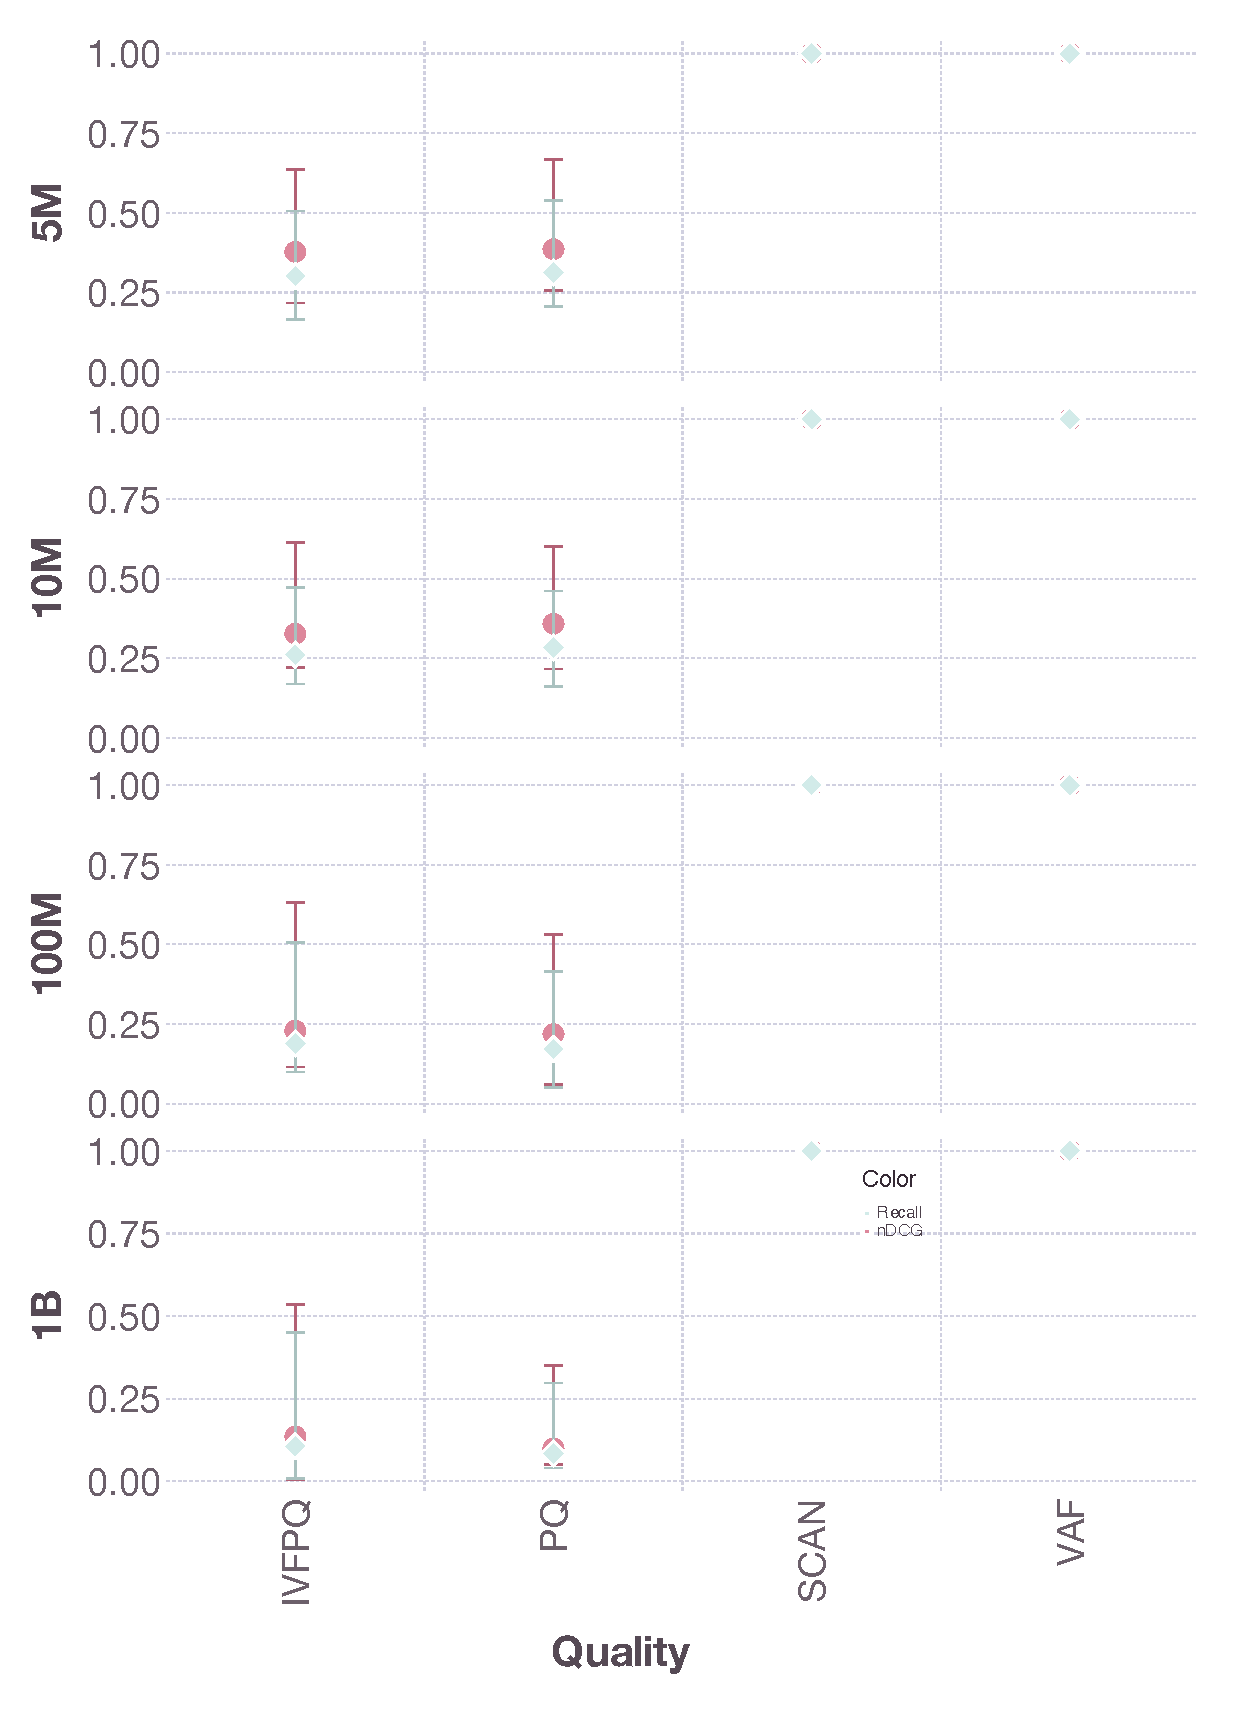
\includegraphics[width=\linewidth]{figures/bignns-cottontail-quality-NNS}
    \caption{Quality metrics for Cottontail DB during the simple \acrshort{nns} large-scale retrieval evaluation presented in \Cref{section:evaluation_bignns_cottontail}. Recall and \acrshort{dcg} are 1.0 for all execution strategies other than \acrshort{pq}, for which they exhibit rather low values with a large spread.}
    \label{figure:appendix_bignns_cottontail_nns_quality}
\end{figure}

\begin{figure}[p]
    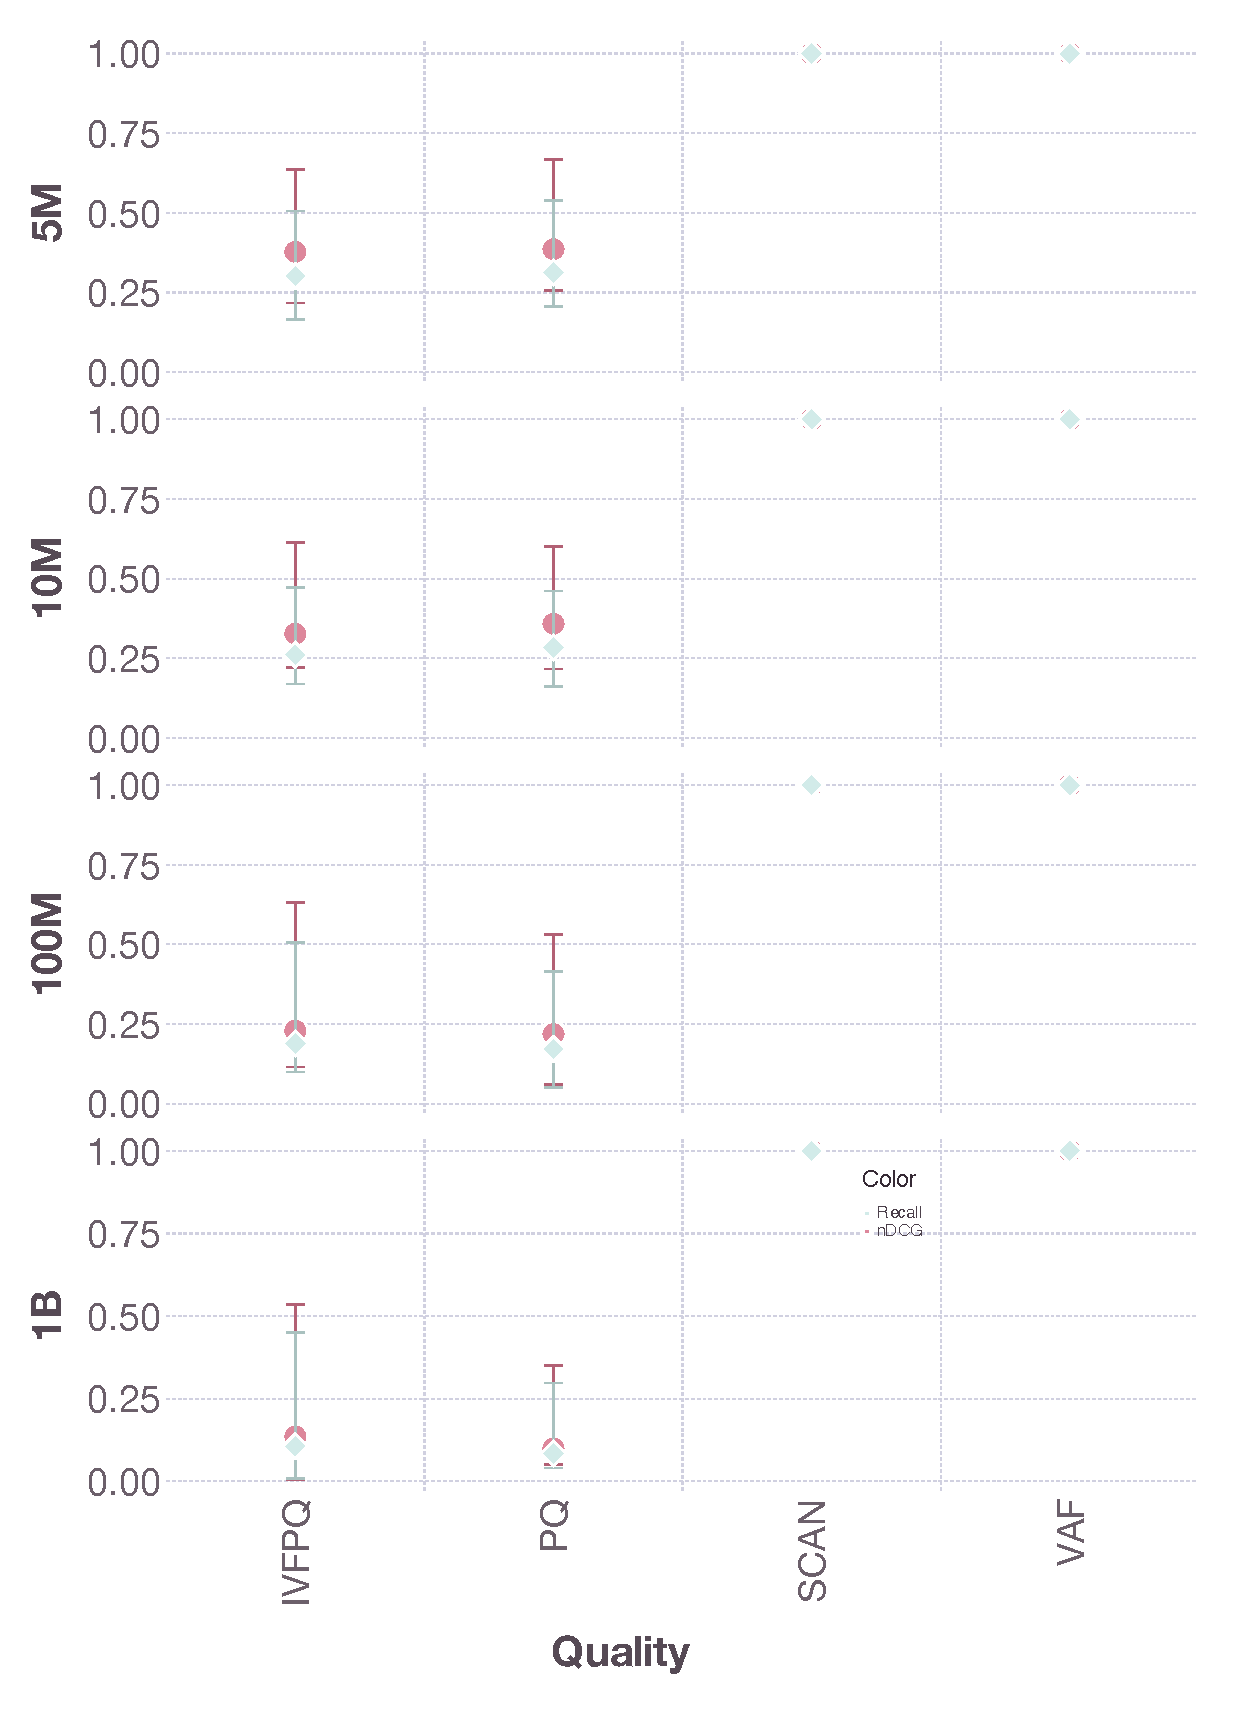
\includegraphics[width=\linewidth]{figures/bignns-cottontail-quality-NNS + Fetch}
    \caption{Quality metrics for Cottontail DB during the \acrshort{nns} + fetch large-scale retrieval evaluation presented in \Cref{section:evaluation_bignns_cottontail}. Recall and \acrshort{dcg} are 1.0 for all execution strategies other than \acrshort{pq}, for which they exhibit rather low values with a large spread.}
    \label{figure:appendix_bignns_cottontail_nns_fetch_quality}
\end{figure}


\begin{figure}[p]
    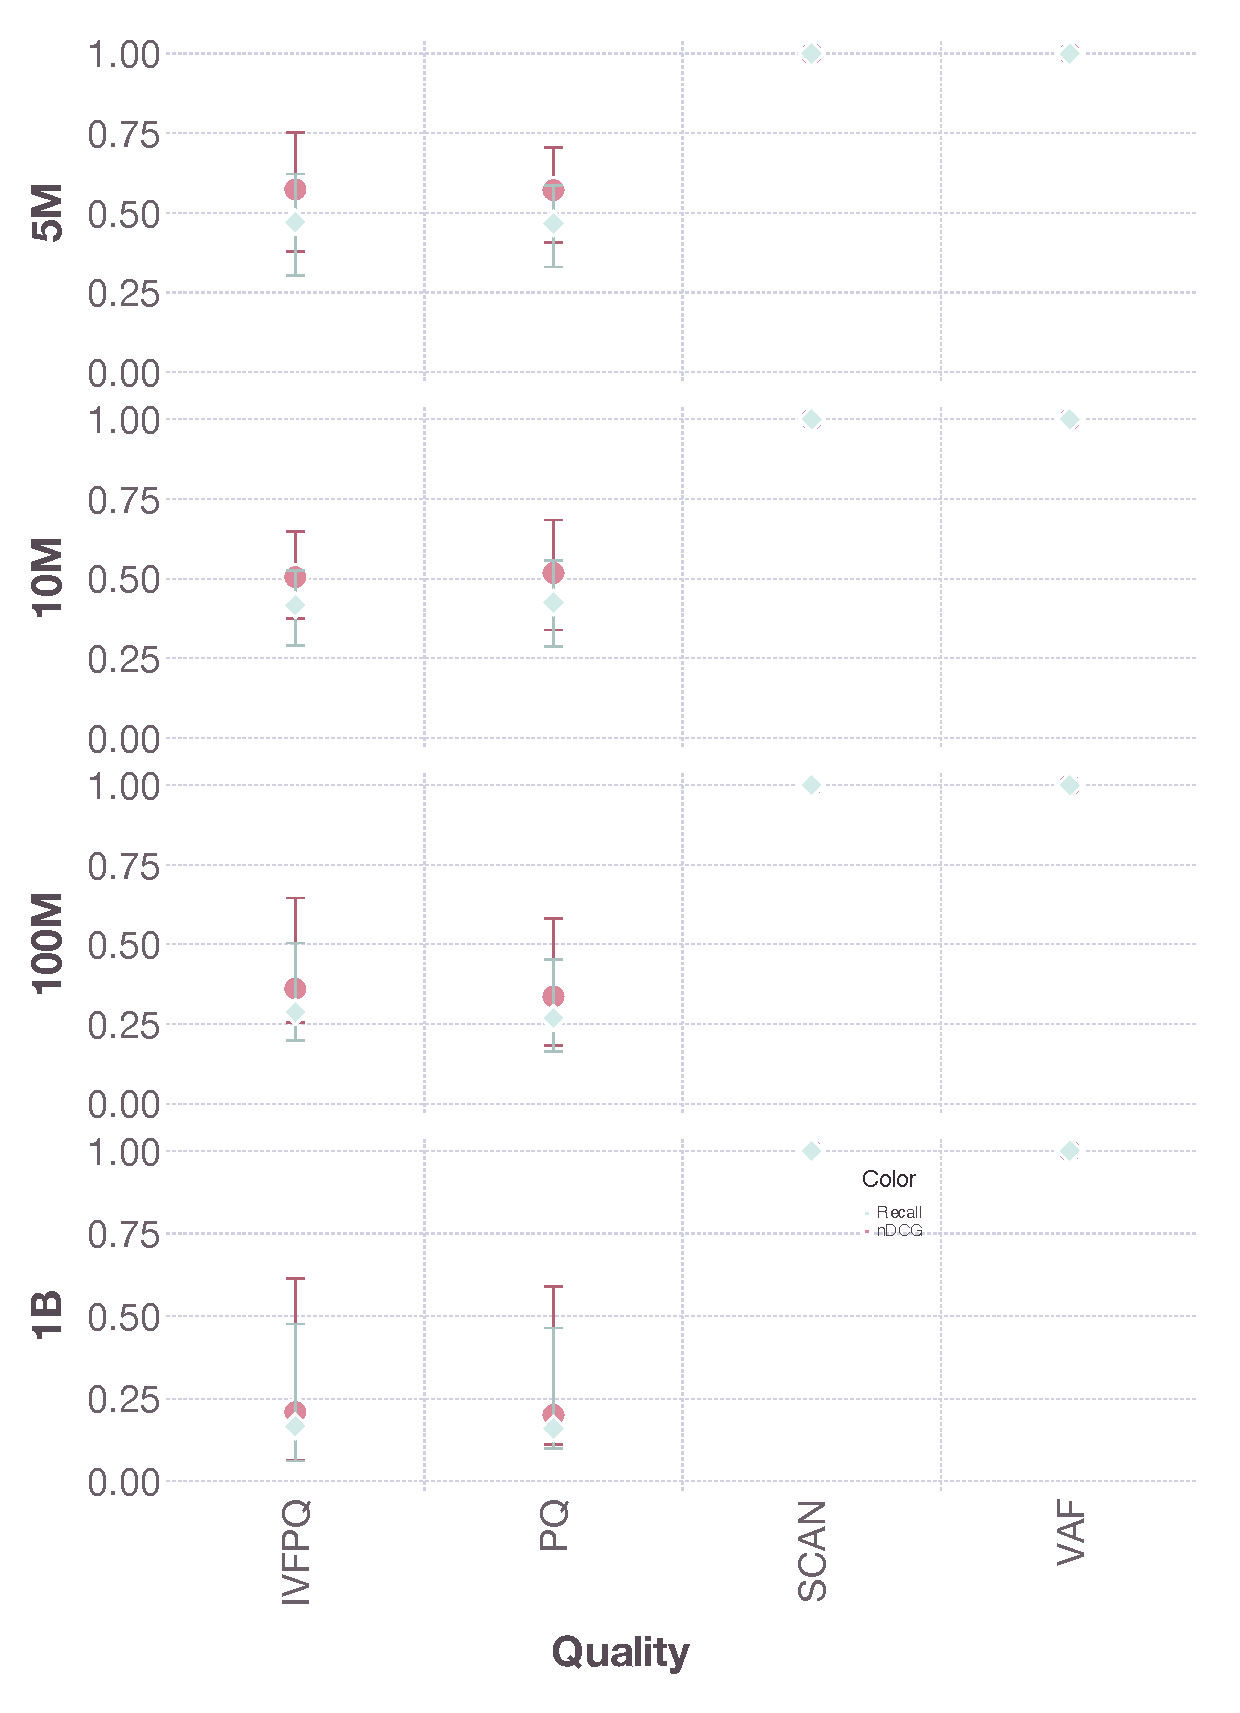
\includegraphics[width=\linewidth]{figures/bignns-cottontail-quality-Hybrid}
    \caption{Quality metrics for Cottontail DB during the hybrid query large-scale retrieval evaluation presented in \Cref{section:evaluation_bignns_cottontail}. Recall and \acrshort{dcg} are 1.0 for all execution strategies other than \acrshort{pq}, for which they exhibit rather low values with a large spread.}
    \label{figure:appendix_bignns_cottontail_hybrid_quality}
\end{figure}
